\section{Study of the ternary representation}

In this section, we study the ternary representation, which is the general representation with weight sharing we obtained above.

\subsection{Genericity}

The ternary representation can represent any kind of layer. For example,
\begin{itemize}
\item To obtain a fully connected layer, one can choose $\omega$ to be of size $nm$ and $S$ the matrix of vectors that contains all possible one-hot vectors.
\item To obtain a convolutional layer, one can choose $\omega$ to be the size of the kernel. $S$ would contain one-hot vectors. A stride $> 1$ can be obtained by removing the corresponding dimensions. If the convolution is a classical convolution, or is supported by a Cayley subgraph (see \chapref{chap:2}), then $S$ would be circulant along the input neurons rank in the canonical basis.
\item Any partially connected layer with (or without) weight sharing can be obtained with appropriate construction of $S$.
\end{itemize}

\subsection{Computationally efficient representation}

\paragraph{What is the fastest way to compute $\Theta S X$ ?}
As the equation \eqref{eq:ternary} is associative and commutative, there are three ways to start to calculate it: with $\Theta S$, $SX$, or $\Theta X$, which we will call \emph{middle-stage tensors}. The computation of a middle-stage tensor is the bottleneck to compute \eqref{eq:ternary} as it imposes to compute significantly more entries than for the second tensor contraction. In \tabref{tab:mid}, we compare their shapes. We refer the reader to \tabref{tab:ind} for the denomination of the indices.

\begin{table}[H]
  \centering
\begin{tabular}{ccc}
  tensor & shape\\
  \hline
  $\Theta$ & $\omega \times P \times Q$\\
  $S$ & $\omega \times n \times m$\\
  $X$ & $n \times P \times B$\\
  $\Theta S$ & $n \times m \times P \times Q$\\
  $SX$ & $\omega \times m \times P \times B$\\
  $\Theta X$ & $\omega \times n \times Q \times B$\\
  $\Theta SX$ & $m \times Q \times B$
\end{tabular}
\caption{Table of shapes}
\label{tab:mid}
\end{table}

In usual settings, we want to have $\omega \ll n$ and $\omega \ll m$, which means that we have weight kernels of small sizes (for example in the case of images, convolutional kernel are of size significantly smaller than that of the images). Also, the number of input channels $P$ and of feature maps $Q$ are roughly in the same order, with $P < Q$ more often than the contrary. It turns out that in practice, the size of $\Theta S$ is significantly bigger than the size of $SX$ and of $\Theta X$, and the size of $SX$ is usually the smallest.

\paragraph{How to exploit $S$ sparsity ?}
Also, in usual settings, $S$ is sparse as $S[:,i,j]$ are one-hot vectors. So computing $SX$ should be faster that computing $\Theta X$, provided we exploit the sparsity. Although $S$ is very sparse as it contains at most a fraction $\frac{1}{w}$-th of non-zero values, it is only sparse along the first rank, which makes implementation with sparse classes of common deep learning libraries not optimized. 

So we proceed differently. The idea is to use a non-sparse tensor $X_{\LRF}$ that has a rank that indexes local receptive fields (LRF), and another rank that indexes elements of these LRF, in order to lower the computation to a dense matrix multiplication (or dense tensor contraction) which is already well optimized. This approach, proposed in \cite{chellapilla2006high}, is also exploited in the cudnn primitives~\citep{chetlur2014cudnn} to efficiently implement the classical convolution.

\paragraph{The LRF representation}
In our case, it turns out that $X_{\LRF}$ can be exactly $SX$, as given fixed~$b$,~$p$, and~$j$, $SX[:,j,p,b]$ corresponds to entries of the input signal $X[:,p,b]$ restrained to a LRF $\ccr_j$ of size~$\omega$. Therefore,
\begin{gather}
\exists \LRF_j = [i_1, \ldots, i_\omega]~\st SX[:,j,p,b] = X[\LRF_j, p, b]
\label{eq:R}
\end{gather}
The elements of $\LRF_j$ can be found by doing a lookup in the one-hot vectors of~$S$, provided each kernel weight occurs exactly once in each LRF. We have:
\begin{gather}
R_j[k] = i_k~\st S[:,i_k,j][k] = 1
\end{gather}
This lookup needs not be computed each time and can be done beforehand. Finally, if we define $\LRF = [\LRF_1, \ldots, \LRF_m]$, \eqref{eq:R} gives:
\begin{gather}
SX = X[\LRF, :, :]
\label{eq:LRF}
\end{gather}
The equation \eqref{eq:LRF} is computed with only $\omega \times m$ assignations and can be simply implemented with automatic differentiation in commonly used deep learning libraries.

\paragraph{Benchmarks}
To support our theoretical analysis, we benchmark three methods for computing the tensor contraction $SX$:
\begin{itemize}
  \item naively using dense multiplication,
  \item using sparse classes of deep learning libraries,
  \item using the LRF based method we described above.
\end{itemize}

We run the benchmarks under the assumptions that $S[:,i,j]$ are one-hot vectors, and that a weight occur exactly once in each LRF (as it is the case for convolutions supported by a Cayley subgraph). For each method, we make $100$ runs of computations of $SX$, with $S$ and $X$ being randomly generated according to the assumptions. In \tabref{tab:ben}, we report the mean time and standard deviation. The values of the hyperparameters were each time $n = m = N = M = B = 100$, and $\omega = 10$. The computations were done on graphical processing units (GPU).

\begin{table}[H]
  \centering
\begin{tabular}{lc}
  Method & Time\\
  \hline
  Naive & \etodo $\mu s~\pm$ \etodo\\
  Sparse & \etodo $\mu s~\pm$ \etodo\\
  LRF & \textbf{\etodo $\mu s~\pm$ \etodo}
\end{tabular}
\caption{Benchmark results}
\label{tab:ben}
\end{table}

As expected, the LRF method is faster.

\subsection{Robustness for extending CNNs}

Intuitively, constructing $S$ amounts, for each LRF, to allocate a different weight to each of its elements. For example, on the pixel domain of images we can obtain the weight sharing scheme $S$ of a classical convolution by moving a rectangular grid, as depicted on \figref{fig:rect}: each point represents the center of of a pixel, and each bin drawn by the rectangular grid is associated with a kernel weight. When the rectangular grid is centered on a point, its LRF is defined by other points falling into a bin, and each bin determines which kernel weight is allocated.

\begin{figure}[H]
      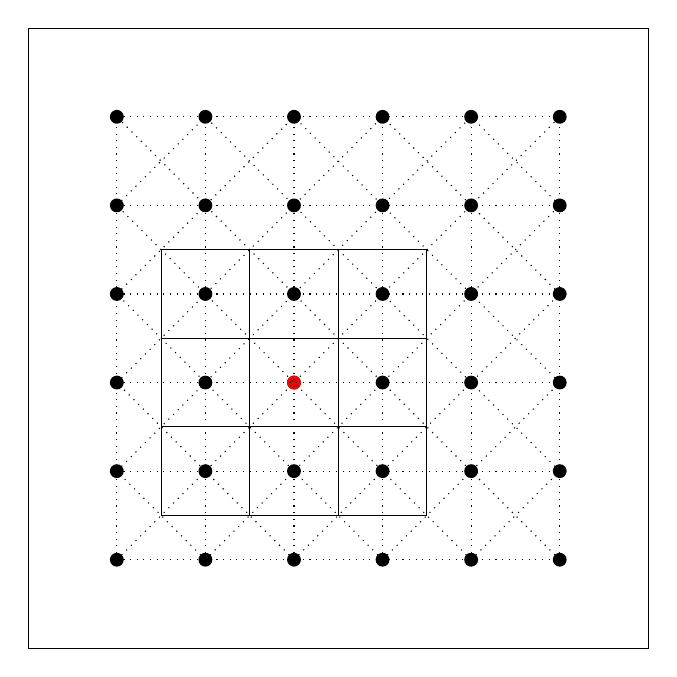
\begin{tikzpicture}[scale=1.125]%[scale=0.75]
        \tikzstyle{every node}= [circle,fill=black, minimum size= 5pt,inner sep=0pt];
          \foreach \x in {1,2,3,4,5,6}{
            \foreach \y in {1,2,3,4,5,6}{
              \node(\x\y) at (\x,\y) {};
            }
          }
          \node(33)[circle,fill=red] at (3,3) {};
          \foreach \x in {1.5,2.5,3.5,4.5}{
            \path[thin]
            (\x,1.5) edge (\x,4.5)
            (1.5,\x) edge (4.5,\x);
          }

          %\draw[ultra thin] (1,6.17) edge[<->] (2,6.17);
          %\node[draw=none,fill=none] at (1.5,6.3) {\scriptsize{$\mu$}};

          \foreach \x in {1,2,3,4,5,6}{
            \draw[dotted,thin] (1,\x) -- (6,\x);
            \draw[dotted,thin] (\x,1) -- (\x,6);
          }

          \foreach \x in {1,2,3,4,5}{
            \draw[dotted,thin] (1,\x) -- (7-\x,6);
            \draw[dotted,thin] (6,\x) -- (\x,6);
          }

          \foreach \x in {2,3,4,5}{
            \draw[dotted,thin] (\x,1) -- (6,7-\x);
            \draw[dotted,thin] (7-\x,1) -- (1,7-\x);
          }

          \draw (0,0) rectangle (7,7);

          %\node[draw=none,fill=none] at (0.9,0.4) {$S=\bbe$};
      \end{tikzpicture}
      \caption{Weight assignement of convolutions on pixel domains}
      \label{fig:rect}
\end{figure}

We are interested in seeing if a 




\begin{figure}[h!t]
      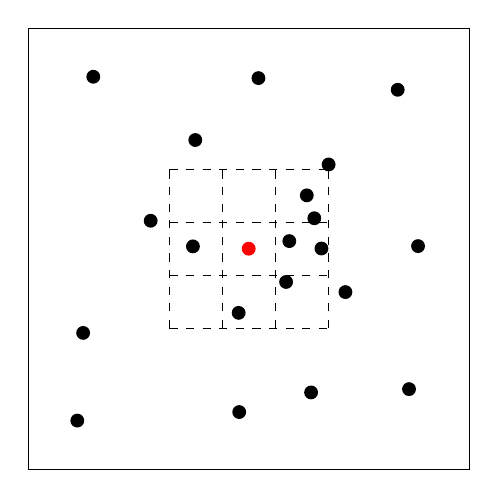
\begin{tikzpicture}[scale=1.12]%[scale=1.055]
        \pgfmathsetseed{5}
        \tikzstyle{every node}= [circle,fill=black, minimum size= 5pt,inner sep=0pt];
        \foreach \x in {1,2,3,4}{
          \foreach \y in {1,2,3,4}{
            \node(\x\y) at (\x+0.5*rand,\y+0.5*rand) {};
          }
        }
        \foreach \y in {1,2,3,4}{
            \node(3\y) at (3+0.5*rand,3+0.5*rand) {};
        }
        \node(33)[circle,fill=red] at (2.5,2.5) {};
        \foreach \x in {1.6,2.2,2.8,3.4}{
          \path[dashed]
          (\x,1.6) edge (\x,3.4)
          (1.6,\x) edge (3.4,\x);
        }

        %\draw[ultra thin] (1.6,1.45) edge[<->] (3.4,1.45);
        %\draw[ultra thin] (2.8,3.55) edge[<->] (3.4,3.55);
        %\node[draw=none,fill=none] at (2.5,1.25) {\scriptsize{$(2p+1)\mu$}};
        %\node[draw=none,fill=none] at (3.15,3.7) {\scriptsize{$\mu$}};

        \draw (0,0) rectangle (5,5);
        %\node[draw=none,fill=none] at (0.7,0.3) {$S=\bbe$};
      \end{tikzpicture}
      \caption{Weight assignement in generalized convolution on distorted domains}
      \label{fig:distrect}
\end{figure}


\subsection{Learning the weight sharing scheme}
